\documentclass[xcolor=pdflatex,dvipsnames,table]{beamer}
\usepackage{epsfig,graphicx}
\usepackage{palatino}
\usepackage{fancybox}
\usepackage{relsize}
\usepackage[procnames]{listings}
\usepackage{hyperref}
\usepackage{qtree} % needed?
\usepackage{booktabs}
\usepackage{dirtree}
\usepackage[normalem]{ulem}


% fatter TT font
\renewcommand*\ttdefault{txtt}
% another TT, suggested by Alex
% \usepackage{inconsolata}
% \usepackage[T1]{fontenc} % needed as well?


\newcommand{\scale}{0.7}

\newcommand{\todo}[1]{{\emph{TODO: #1}}}
\newcommand{\martin}[1]{{\color{blue} Martin: #1}}
\newcommand{\abcdef}[1]{{\color{red} Author2: #1}}

% uncomment following for final submission
%\renewcommand{\todo}[1]{}
%\renewcommand{\martin}[1]{}
%\renewcommand{\author2}[1]{}

\newcommand{\code}[1]{{\texttt{#1}}}

\hypersetup{
  linkcolor  = black,
%  citecolor  = blue,
  urlcolor   = blue,
  colorlinks = true,
}

\beamertemplatenavigationsymbolsempty
\setbeamertemplate{footline}[frame number]





\newif\ifbook
% shared in slides and book

\lstdefinelanguage{chisel}{
  morekeywords={abstract,case,catch,class,def,%
    do,else,extends,false,final,finally,%
    for,if,implicit,import,match,mixin,%
    new,null,object,override,package,%
    private,protected,requires,return,sealed,%
    super,this,throw,trait,true,try,%
    type,val,var,while,with,yield},
  otherkeywords={=>,<-,<\%,<:,>:,\#,@},
  sensitive=true,
  morecomment=[l]{//},
  morecomment=[n]{/*}{*/},
  morestring=[b]",
  morestring=[b]',
  morestring=[b]"""
}

\usepackage{color}
\definecolor{dkgreen}{rgb}{0,0.6,0}
\definecolor{gray}{rgb}{0.5,0.5,0.5}
\definecolor{mauve}{rgb}{0.58,0,0.82}

% Default settings for code listings
\ifbook
\lstset{%frame=lines,
  language=chisel,
  aboveskip=3mm,
  belowskip=3mm,
  showstringspaces=false,
  columns=fixed, % basewidth=\mybasewidth,
  basicstyle={\small\ttfamily},
  numbers=none,
  numberstyle=\footnotesize,
  % identifierstyle=\color{red},
  breaklines=true,
  breakatwhitespace=true,
  procnamekeys={def, val, var, class, trait, object, extends},
  % procnamestyle=\ttfamily,
  tabsize=2,
  float
}
\else
\lstset{%frame=lines,
  language=chisel,
  aboveskip=3mm,
  belowskip=3mm,
  showstringspaces=false,
  columns=fixed, % basewidth=\mybasewidth,
  basicstyle={\small\ttfamily},
  numbers=none,
  numberstyle=\footnotesize\color{gray},
  % identifierstyle=\color{red},
  keywordstyle=\color{blue},
  commentstyle=\color{dkgreen},
  stringstyle=\color{mauve},
  breaklines=true,
  breakatwhitespace=true,
  procnamekeys={def, val, var, class, trait, object, extends},
  procnamestyle=\ttfamily\color{red},
  tabsize=2,
  float
}
\fi

\lstnewenvironment{chisel}[1][]
{\lstset{language=chisel,#1}}
{}

\newcommand{\shortlist}[1]{{\lstinputlisting[nolol]{#1}}}

\newcommand{\longlist}[3]{{\lstinputlisting[float, caption={#2}, label={#3}, frame=tb, captionpos=b]{#1}}}

\newcommand{\verylonglist}[3]{{\lstinputlisting[caption={#2}, label={#3}, frame=tb, captionpos=b]{#1}}}


\title{Finite State Machine with Datapath}
\author{Martin Schoeberl}
\date{\today}
\institute{Technical University of Denmark\\
Embedded Systems Engineering}

\begin{document}

\begin{frame}
\titlepage
\end{frame}


\begin{frame}[fragile]{TODO}
\begin{itemize}
\item Repeat the testing including showing it on the screen
\item Try it out with some
\item Also input processing (maybe)
\item add cosimulation to the verification story (show Lipsi), maybe later
\item logic gen., maybe bin bcd directly into vec
\end{itemize}
\end{frame}

\begin{frame}[fragile]{Overview}
\begin{itemize}
\item Remote teaching and learning
\item Repeat
\item FSM with Datapaht
\end{itemize}
\end{frame}

\begin{frame}[fragile]{Remote Learning}
\begin{itemize}
\item First: this is all new for the most of us
\begin{itemize}
\item We need to be patient with each other
\end{itemize}
\item We should use Slack for quicker communication
\item Zoom for lecturing
\begin{itemize}
\item \url{https://dtudk.zoom.us/j/7712109832}
\end{itemize}
\item Please use a headset
\item Please mute your mic when not talking
\item Some nice features
\begin{itemize}
\item You can raise your hand
\item You can ask questions with mic or on chat
\item Everyone can share their screen or an individual window
\end{itemize}
\item The Dally book is now available online for free!
\end{itemize}
\end{frame}

\begin{frame}[fragile]{Lab/Exercise Organization}
\begin{itemize}
\item Everyone at DTU can use the professional version of Zoom
\begin{itemize}
\item \url{http://dtudk.zoom.us/signin}
\end{itemize}
\item You can also use Zoom for your group work
\item Zoom will also be used for the supervised lab
\begin{itemize}
\item Start a Zoom meeting with your group
\item Schedule a TA for help with Slack, posting your Zoom meeting link
\item You can also schedule a Zoom meeting with me (also at other times)
\end{itemize}
\item This is a chance to learn how to collaborate remotely
\begin{itemize}
\item This will be part of your future work as engineer anyway
\end{itemize}
\item This experiment might change how we teach in the future
\end{itemize}
\end{frame}

\begin{frame}[fragile]{Lab Work}
\begin{itemize}
\item We will stick to the plan of a working Vending Machine
\begin{itemize}
\item At the end it shall run in your FPGA board
\item I am a big fan of running stuff in real hardware
\end{itemize}
\item Demo your work to a TA via the camera
\item I know many groups have only one physical FPGA board
\item A lot can be done in simulation
\item I plan to develop a simulation of the Basys3 board
\item I assume you have found a solution for file sharing
\begin{itemize}
\item GitHub is a popular one for source code
\item Can also be used if you plan to write your report in LaTeX
\end{itemize}
\end{itemize}
\end{frame}

\begin{frame}[fragile]{Questions?}
\begin{itemize}
\item On lectures
\item On the group/lab work
\end{itemize}
\end{frame}

\begin{frame}[fragile]{FSM with Datapath}
\begin{itemize}
\item A type of computing machine
\item Consists of a finite-state machine (FSM) and a datapath
\item The FSM is the master (the controller) of the datapath
\item The datapath has computing elements
\begin{itemize}
\item E.g., adder, incrementer, constants, multiplexers, ...
\end{itemize}
\item The datapath has storage elements (registers)
\begin{itemize}
\item E.g., sum of money payed, count of something, ...
\end{itemize}
\end{itemize}
\end{frame}

\begin{frame}[fragile]{FSM-Datapath Interaction}
\begin{itemize}
\item The FSM controls the datapath
\begin{itemize}
\item For example, add 2 to the sum
\end{itemize}
\item By controlling multiplexers
\begin{itemize}
\item For example, select how much to add
\item Not adding means selecting 0 to add
\end{itemize}
\item Which value goes where
\item The FSM logic also depends on datapath output
\begin{itemize}
\item Is there enough money payed to release a can of soda?
\end{itemize}
\item FSM and datapath interact
\end{itemize}
\end{frame}


\begin{frame}[fragile]{Popcount Example}
\begin{itemize}
\item An FSMD that computes the popcount
\item Also called the Hamming weight
\item Compute the number of `1's in a word
\item Input is the data word
\item Output is the count
\item Code available at \href{https://github.com/schoeberl/chisel-book/blob/master/src/main/scala/PopCount.scala}{PopCount.scala}
\end{itemize}
\end{frame}

\begin{frame}[fragile]{Popcount Block Diagram}

\begin{figure}
  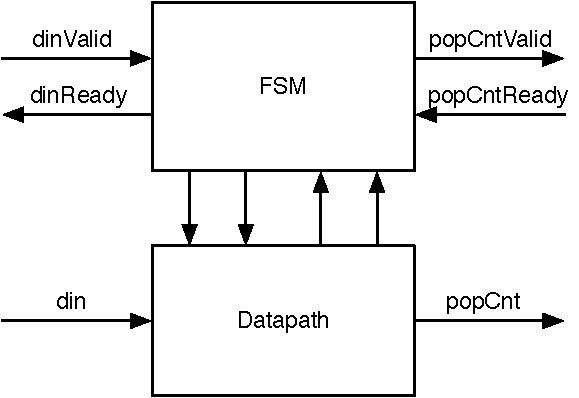
\includegraphics[scale=\scale]{../figures/popcnt-fsmd}
\end{figure}
\end{frame}


\begin{frame}[fragile]{Popcount Connection}
\begin{columns}
\column{0.6\textwidth}
\begin{itemize}
\item Input \code{din} and output \code{popCount}
\item Both connected to the datapath
\item We need some handshaking
\item For data input and for count output
\end{itemize}
\column{0.4\textwidth}
\begin{figure}
  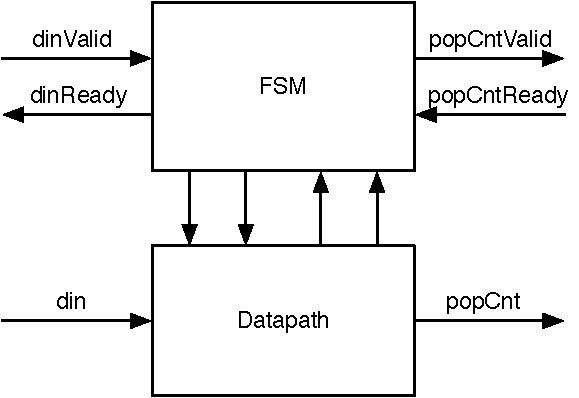
\includegraphics[scale=0.45]{../figures/popcnt-fsmd}
\end{figure}
\end{columns}
\end{frame}

\begin{frame}[fragile]{Popcount Handshake}
\begin{columns}
\column{0.6\textwidth}
\begin{itemize}
\item We use a ready-valid handshake
\item When data is available valid is asserted
\item When the receiver can accept data ready is asserted
\item Transfer takes place when both are asserted
\end{itemize}
\column{0.4\textwidth}
\begin{figure}
  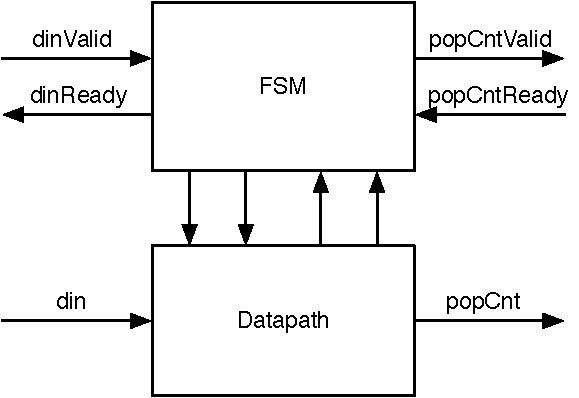
\includegraphics[scale=0.45]{../figures/popcnt-fsmd}
\end{figure}
\end{columns}
\end{frame}


\begin{frame}[fragile]{The FSM}
\begin{figure}
  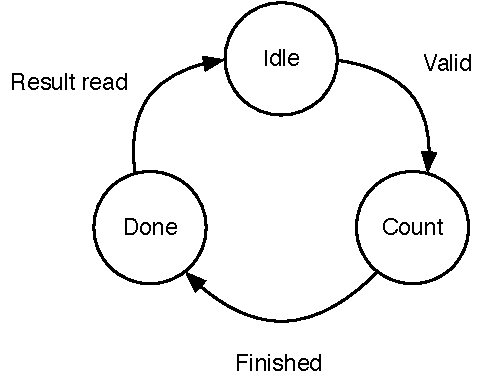
\includegraphics[scale=\scale]{../figures/popcnt-states}
\end{figure}
\begin{itemize}
\item A Very Simple FSM
\item Two transitions depend on input/output handshake
\item One transition on the datapath output
\end{itemize}
\end{frame}

\begin{frame}[fragile]{xxx}
\begin{itemize}
\item yyy
\end{itemize}
\end{frame}

\begin{frame}[fragile]{Usage of an FSMD}
\begin{itemize}
\item Maybe your vending machine is an FSMD?
\end{itemize}
\end{frame}


\begin{frame}[fragile]{xxx}
\begin{itemize}
\item yyy
\end{itemize}
\end{frame}

\begin{frame}[fragile]{Today Lab}
\begin{itemize}
\item Paper \& pencil exercises
\item Exercises on FSM
\item From the, now free, Dally book
\end{itemize}
\end{frame}

\begin{frame}[fragile]{Summary}
\begin{itemize}
\item We ave interesting teaching constraints
\item We will still be able to build a vending machine
\end{itemize}
\end{frame}


\end{document}

%\begin{frame}[fragile]{xxx}
%\begin{itemize}
%\item yyy
%\end{itemize}
%\end{frame}
